\documentclass[12pt,fleqn]{article}\usepackage{../common}
\begin{document}
Ders 5

Permutasyonlar

Bu derste bir anlamda lineer cebirin ruhunu gormeye baslayacagiz, sadece
vektorler degil artik vektor uzaylarina bakmaya baslayacagiz, yani daha
buyuk resme odaklanacagiz. Ayrica herhangi bir uzayin alt-uzaylarini
(subspace) inceleyecegiz. 

Permutasyonlari hatirlayalim: permutasyon matrisi $P$ bir diger matrisin
satirlarini degis-tokus etmek icin kullaniliyordu. Bu isleme ihtiyacimiz
olabilir, cunku, elimizde $Ax=b$ cozerken belki de (neredeyse) mukemmel bir
$A$ olsa da bazen mesela tek bir yerdeki sifir isi bozuyor olabilir, onu
yerinden oynatirsam, duzgun bir pivot elde edersem cozum olacaktir, iste o
zaman permutasyon kullanabilirim.

Peki $A=LU$'nun bir sistemi cozerken gerekebilecek permutasyonlar ile
alakasi nedir?

$A=LU$'nin ne oldugunu hatirlayalim, 

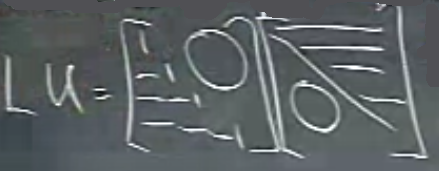
\includegraphics[height=3cm]{5_01.png}

Bu resme bakarsa, bu tur gosterilen bir $LU$ tarifi $P$'nin olmadigini
farz ediyor, yani hic satir degis-tokusuna gerek olmadigi farz
ediliyor. Peki eger satir degis tokusu gerekseydi, bu durumu cebirsel
olarak nasil gosterirdim?

Aslinda ustteki tanimda da $P$ ``var'', ya da oldugunu dusunebiliriz, ama
$P$ bu durumda birim matrisidir. 

Simdi bir dakika durup mesela Matlab [artik Python] lineer cebir
kutuphanelerinin cozumu nasil yaptigini dusunelim. Bu kutuphaneler pivot'in
sifir olup olmadigina bakarlar, ki herhangi bir insan da bunu yapar, ayrica
pivot'in ``yeterince buyuk olup olmadigina da'' bakilir, cunku sifira
yakin, cok kucuk pivotlar sayisal hesap baglaminda kotudur. Bu durumda
kutuphaneye ``coz'' dedigimizde kodun arka planda satir degis-tokuslari
yaptigini gorururuz, bu degisimler pur matematiksel olarak gerekli
olmayabilirler, ama hesap / sayisal acidan gereklidirler. 

Neyse, ya sayisal sebepten, ya da baska bir sebepten dolayi satir degis
tokusu gerekebilir, o zaman nihai olarak satir degisimini iceren
eliminasyon sudur:

$$ PA = LU $$

$P$ satir degis-tokusunu yapan matristir. $P$, $A$'yi ``ideal'' hale
getirir, sifirlar pivot'ta olmaz, vs. 

Bu arada bir permutasyon matrisinin yapisini hatirlayalim, temelinde bir
permutasyon matrisi satirlarinin yeri degistirilmis bir birim
matristir. Permutasyon matrisleri pek cok satir degisimi ayni anda
yapabilir, kac turlu degisim kombinasyonu vardir? 

$$ n! = n(n-1)...(3)(2)(1) $$

cunku ustteki kadar degisik satir siralamasi mumkundur, ve tum
permutasyonlari boyle hesaplayabiliriz. 

Ayrica $P$ tersi alinabilir (invertible) bir matristir, ve 

$$ P^{-1} = P^T $$

ya da 

$$ P^TP = I $$

Bu ``guzel'' bir ozellik, ve bu tur ozelliklere sahip olan matrisler bizi
ozellikle ilgilendiriyor.

Ornek

$$ 
\left[\begin{array}{rr}
1 & 3 \\
2 & 3 \\
4 & 1 
\end{array}\right]^T
 $$

Basit bir devrik islemi... Sonuc nedir?

$$ =
\left[\begin{array}{rrr}
1 & 2 & 4 \\
1 & 3 & 3 
\end{array}\right]
 $$

Devrik islemi, formulsel olarak 

$$ (A^T)_{ij} = A_{ji} $$

Simdi simetrik matrislerden bahsedelim, bunlar cok ``sevdigimiz''
matrislerden biri. Bu matrislerin guzel bir ozelligi, devrigi kendisine
esit olmasi,

$$ A^T = A $$

Mesela

$$ 
\left[\begin{array}{rrr}
3 & 1 & 7 \\
1 & 2 & 9 \\
7 & 9 & 4
\end{array}\right]
 $$

Bu tur bir matrisi ne zaman elde ederiz? Iki ustteki matris mesela $3
\times 2$ boyutunda zaten, simetrik olmasi zaten mumkun degil, cunku devrik
islemi boyut degisikligine sebep oluyor. Fakat dikdortgensel olsa bile
(cunku kare seklinde degil, yani boyutlari farkli) bir matristen acaba bir
islem uyguluyarak simetrik bir matris elde edemez miyim? Fikir: iki ustteki
matrise $R$ diyelim, $R^TR$ ile simetrik bir matris elde edebilirim. Bu
hakikaten mumkun, hatta kural olarak alabiliriz, $R^TR$ her zaman simetrik
matris verir. Ornekte gorelim, 

$$ 
\left[\begin{array}{rr}
1 & 3 \\
2 & 3 \\
4 & 1 
\end{array}\right]^T
\left[\begin{array}{rrr}
1 & 2 & 4 \\
1 & 3 & 3 
\end{array}\right]
=
\left[\begin{array}{rrr}
10 & 11 & 7 \\
11 & .. & .. \\
7 & .. & ..
\end{array}\right]
 $$  

Gerisi de ayni olacakti. Sembolik olarak gorelim, $R^TR$'in simetrik
oldugunu nasil bulurum? Onun devrigini alabilirim, ve sonucun degismemesini
kontrol edebilirim,

$$ (R^TR)^T = R^T(R^T)^T $$

$(R^T)^T$ nedir? Bir matrisin iki kere devrigini alirsam tekrar kendisine
donmus olmaz miyim? Evet. O zaman, 

$$  R^T(R^T)^T = R^T R $$

Bastaki hale donduk! Demek ki $R^TR$ bir simetrik matristir. Ispat
tamamlandi. 

Vektor Uzaylari

Vektorlerle ne islemleri yaptigimizi dusunelim. Onlari topluyoruz mesela,
ya da onlari bir skalar (yani tek sayi) ile carpiyoruz... Bir uzayin vektor
uzayi olarak kabul edilmesi icin bu tur islemlerin ``aile icinde''
kalabilmesi gerekir, yani toplam, carpim islemlerinin sonuclari da uzay
icinde yer almali. 

Ornek

Icinde tum 2 boyutlu vektorleri iceren $ \mathbb{R}^2 $. Sembol
$\mathbb{R}$'i gorunce reel sayilar anliyoruz, yani reel sayilar ama onun
iki boyutlu hali.

$$ 
\left[\begin{array}{r}
3 \\ 2 
\end{array}\right], 
\left[\begin{array}{r}
0 \\ 0
\end{array}\right], 
\left[\begin{array}{r}
\pi \\ e
\end{array}\right], 
..
 $$

Diger yonden soyle gorebiliriz, $\mathbb{R}^2$ tum $x-y$ duzlemidir. Ve bu
duzlem bu uzay bir vektor uzayidir. Niye? Cunku ihtiyacimiz olan tum
noktalar oradadir, orijin bile, oradadir ve ona ihtiyac vardir. Farz
edelim orijin noktasini bu uzaydan cikardim, yani $x-y$ duzleminin sanki
ortasina bir delik actim. Fakat vektor uzayi tanimina gore herhangi bir
vektoru istedigim bir skalar ile carpabilmeliyim, sifirla da
carpabilmeliyim ve sonuc bu durumda orijin olacaktir, ama orijin uzayda
yoksa erisebilecegim her turlu sonucu icermedigi icin bu bir vektor uzayi
olamaz. Ya da $\left[\begin{array}{rr}3 & 2\end{array}\right]^T$ vektorune$[-3 \ -2]^T$ ekleyebilmeliyim, ve sonuc yine 
orijin olacak, ama  yoksa problem cikar.

Eger $\mathbb{R}^3$ kullansaydik, bu icinde tum 3 boyutlu reel vektorleri
iceren uzay olurdu. 

Ya $\mathbb{R}^n$? Icinde $n$ tane reel sayi olan, $n \times 1$ boyutunda
kolon vektorleri. 

Baska bir ornek gorelim, mesela alttaki durum. Burada sadece $x-y$
duzleminin sag ust tarafindaki (altta isaretli) alani bir uzay olarak almak
istedik. 

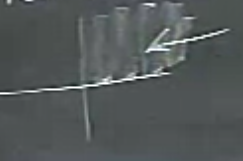
\includegraphics[height=4cm]{5_02.png}

Soru su: bu bir uzay midir? Yani icindeki vektorlerin tum lineer
kombinasyonun yine kendisi icinde midir? 

Eger oradaki bir vektoru, mesela $\left[\begin{array}{rr}3 &
    2\end{array}\right]^T$ alip bir diger vektorle toplarsam mesela
$\left[\begin{array}{rr}6 & 8\end{array}\right]^T$ sonuc hala bu ust sag kosede olur. Problem bir skalar ile carptigimizda ortaya cikar; eger
$\left[\begin{array}{rr}3 & 2\end{array}\right]^T$ alip $-3$ ile carparsam, sonuc eksi yone isaret eden bir vektor olur, o zaman sag ust kosenin disina
tasmis olurum. Yani tanimladigim alan carpma islemi icin ``kapali'' (closed) degildir.
O zaman bu bir vektor uzayi degildir. 

Ustteki ornekte mevcut bir vektor uzayinin bir kismini aldik, ve vektor
uzayi olmadigini gorduk. Peki tum alt uzaylar (subspace) bu sekilde vektor
uzayi degil midir? $\mathbb{R}^2$'ye donelim, onun bir alt uzayina
bakalim. 

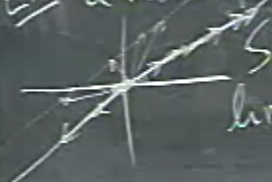
\includegraphics[height=4cm]{5_03.png}

Eger orijinden gecen ve yukari asagi sonsuza giden capraz bir cizgi cizsem,
bu cizgi bir vektor uzayi olan alt uzay olur muydu? Evet. Niye? Cunku onun
uzerindeki herhangi iki vektoru birbirine toplasam yine ayni cizgi uzerine
olurum [hoca bunu gostermek icin bir suru oklar cizdi ayni cizgi
uzerinde]. Eger sag yukari giden bir vektoru negatif bir skalar ile carpsam
ters yone giderim ama problem degil, bu yon de mevcut. Unutmayalim, tek
sayi ile carpinca yonu degistirebiliriz, ama 180 derece terse gidebiliriz
sadece, azicik daha yukari ya da asagi gidemeyiz. Demek ki hep ayni cizgi
uzerindeyiz. 

Tabii eklemeye gerek yok, orijin muhakkak uzayin icinde olmali, yoksa sifir
ile carpinca orijin sonucu gelir, ama o nokta uzayda degilse yine ``disari
tasmis'' olurum. Mesela 

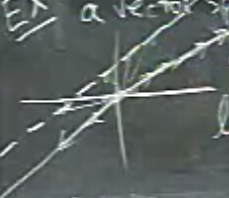
\includegraphics[height=4cm]{5_04.png}

oncekine paralel [kesik cizgiyle gosteriliyor] yeni bir cizgi cizdim
mesela. Bu cizgi bir vektor uzayi degildir, cunku sifirla carpinca orijin
sonucu cikar, bu nokta o kesikli olan uzayda yoktur.

Bu arada $\mathbb{R}^2$'de iken kendimize su soruyu soralim; kac tane
farkli alt mumkundur? 

1) $\mathbb{R}^2$'nin kendisi (o da bir alt-uzay)

2) Orijinden gecen her cizgi. Dikkat, bir cizgiden bahsedince ve bu cizgi
tek yonde olunca, akla ``acaba bu cizgi $\mathbb{R}^1$ mi?'' sorusu
gelebilir. Bu alt uzay $\mathbb{R}^1$ degil, $\mathbb{R}^1$ olsaydi icinde
iki degil tek sayi olan bir ``vektorden'' bahsediyor olurduk. 

3) Icinde sadece sifir vektor olan bir uzay - ki ben buna cogu zaman
$\mathbb{Z}$ diyorum. Bu mantikli degil mi? Sifir vektoru aliyorum,
kendisiyle topluyorum, ayni uzaydayim. Herhangi bir skalar ile carpiyorum,
mesela 17, sifir carpi herhangi bir baska sey sifir olduguna gore, yine
ayni uzaydayim! Oyle degil mi? $\left[\begin{array}{rr}0 &
    0\end{array}\right]^T \cdot 17 = \left[\begin{array}{rr}0 &
    0\end{array}\right]^T$.

Peki $\mathbb{R}^3$'un kac alt uzayi vardir? Yine $\mathbb{R}^3$'un
kendisi, orijin noktasi, ve orijinden gecen tum duzlemler (planes). Ya da
orijinden gecen tum cizgiler. 

Matrislerin Alt Uzayi

Ustteki ornek alt uzaylar $\mathbb{R}^2$, k$\mathbb{R}^3$'ten
geldiler. Acaba bir matristen bir alt uzay yaramaz miyiz? Mesela 

$$  A =
\left[\begin{array}{rr}
1 & 3 \\
2 & 3 \\
4 & 1 
\end{array}\right]
 $$

matrisinin alt uzayi nedir? 

$A$'nin kolonlarina bakiyorum, bu kolonlar $\mathbb{R}^3$ icindeler. Ve bir
alt uzay yaratiyorum, o zaman bu kolonlarin o alt uzay icinde olmasini
isterim. Fakat bir alt uzaya iki tane kolon atip ``iste bu bir alt uzay''
diyemem. Oraya baska ne koymam lazim? Bu iki kolonun her turlu lineer
kombinasyonu orada olmali, mesela $ \left[\begin{array}{rrr}4 & 5 &
    5\end{array}\right]^T$ orada olmali o zaman, ya da sifirla carpacagim,
$\mathbb{Z}^3$ orada olmali, vs. Ya da ilk kolondan bir tane, ikincisinden
uc tane alip toplayacagim, bu sonucun da uzay olmasi gerekir. 

Eger tum bunlari yaparsam bir alt uzay yaratmis olurum, ki matris
baglaminda bu uzaya ``kolon uzayi (columnspace)'' ismi de verilir. Buna
$C(A)$ diyelim. 

Bu aradigimiz uzay nasil bir sey olur acaba? Iki vektor var, onlarin tum
kombinasyonlari ayni uzay icinde kalacak, ve orijin dahil
olacak.. Geometrik olarak dusunelim,

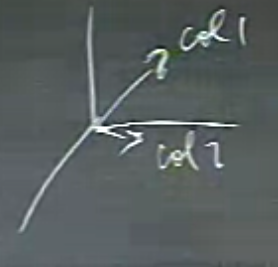
\includegraphics[height=4cm]{5_05.png}

iki vektoru boyle cizdik diyelim. Bu her iki vektoru icinde barindiran, ve
her turlu kombinasyonunu da iceren sey nedir? Bu sey her ne ise, herhalde
bir cizgi olamaz, cunku basit bir kac ornekle tamamen farkli yonlere isaret
eden kombinasyonlar bulabiliriz, ayrica bu her iki vektoru uzerinde tutan
bir cizgi zaten mumkun degil. O zaman ne? 

Bir duzlem! Her iki vektoru de uzerinde barindiran ve orijinden gecen
duzlem bir alt uzaydir.

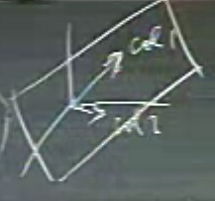
\includegraphics[height=4cm]{5_06.png}

Degil mi? Bu iki vektorun her turlu kombinasyonu bu duzlem uzerindedir. Bu
kritik bir bulgu - uzerinde iyice dusunelim. Gorelim. Tabii 3 boyutta
gorebiliriz, ama $\mathbb{R}^{10}$ boyutunda da is yapacagiz, ve bu uzayda
diyelim 5 tane vektorun kombinasyonunu aliyoruz, ki bu bir alt uzay
yaratir, [hoca neredeyse $\mathbb{R}^5$'i gorsel olarak tarif etmek ister
gibi yapti, ama bu uzayi gorsel olarak dusunmek mumkun degil, bilemeyiz
dedi], 5 vektor ki her birinin 10 tane ogesi var, bunlarin kombinasyonunu
aliyoruz, sonuc olarak, dikkat, $\mathbb{R}^5$'te degiliz cunku elimizde 10
ogeli vektorler var. Buyuk ihtimalle bu kombinasyon bir duzlemde olacak,
ama.. yani eger vektorler o sekilde ise bir cizgi de ortaya
cikabilir. Anlatabiliyor muyum? Her sey o 5 vektorun ne olduguna bagli. 

Ayni sekilde, bir onceki ornekte, eger iki vektor bir cizgi uzerinde
olsaydi, onlarin kolon uzayi o cizgi olurdu (ama ornekte alt uzay bir
duzlem haline geldi). 

Bu noktada duralim; bir sonraki derste $Ax=b$'yi biraz once belirttigim dil
ile nasil gorurum, ona bakacagiz. Bu dilde kolon uzaylari, vektor uzaylari
var, bunlar $Ax=b$ ile nasil baglantili. Baska ne tur uzaylar vardir? Iki
tanesini gorduk, baska turleri de var. 

\end{document}
